\documentclass[11pt]{article}

%% Language and font encodings
\usepackage[english]{babel}
\usepackage[utf8]{inputenc}
\usepackage[T1]{fontenc}
\usepackage{textcomp}
\usepackage{biblatex}

\usepackage{graphicx}
\usepackage{amsmath,mathtools,amssymb}


%%%%%%%%%%%%%%%%%%%
% aliases
%%%%%%%%%%%%%%%%%%%

\newcommand{\T}[2]{\prescript{#1}{}{\bfT}_{#2}}
% \newcommand{\Th}[2]{\prescript{#1}{}{\widehat T}_{#2}}  % ?
\newcommand{\Tm}[2]{\prescript{#1}{}{\widetilde{\bfT}}_{#2}}
\newcommand{\Rot}[2]{\prescript{#1}{}{\bfR}_{#2}}
\newcommand{\Rotm}[2]{\prescript{#1}{}{\widetilde{\bfR}}_{#2}}
\newcommand{\noise}{\bfn}
\newcommand{\bias}{\bfb}

\newcommand{\posiv}[1]{\underline{\bfp}_{#1}}
\newcommand{\posi}[2]{\prescript{#1}{}{\bfp}_{#2}}
\newcommand{\posim}[2]{\prescript{#1}{}{\widetilde{\bfp}}_{#2}}
\newcommand{\posibar}{\bar{\bfp}}
\newcommand{\velv}[1]{\underline{\bfv}_{#1}}
\newcommand{\vel}[2]{\prescript{#1}{}{\bfv}_{#2}}
\newcommand{\velm}[2]{\prescript{#1}{}{\widetilde{\bfv}}_{#2}}
\newcommand{\accv}[1]{\underline{\bfa}_{#1}}
\newcommand{\acc}[2]{\prescript{#1}{}{\bfa}_{#2}}
\newcommand{\accm}[2]{\prescript{#1}{}{\widetilde{\bfa}}_{#2}}
\newcommand{\angvelv}[1]{\underline{\pmb{\omega}}_{#1}}
\newcommand{\angvel}[2]{\prescript{#1}{}{\pmb{\omega}}_{#2}}
\newcommand{\angvelm}[2]{\prescript{#1}{}{\widetilde{\pmb{\omega}}}_{#2}}
\newcommand{\angvelbar}{\bar{\pmb{\omega}}}
\newcommand{\forcev}[1]{\underline{\bff}_{#1}}
\newcommand{\force}[2]{\prescript{#1}{}{\bff}_{#2}}
\newcommand{\forcem}[2]{\prescript{#1}{}{\widetilde{\bff}}_{#2}}
\newcommand{\torquev}[1]{\underline{\pmb{\tau}}_{#1}}
\newcommand{\torque}[2]{\prescript{#1}{}{\pmb{\tau}}_{#2}}
\newcommand{\torquem}[2]{\prescript{#1}{}{\widetilde{\pmb{\tau}}}_{#2}}

\newcommand{\AM}{\mathcal{L}}
\newcommand{\AMv}{\underline{\mathcal{L}}}
\newcommand{\AMm}{\widetilde{\mathcal{L}}}
\newcommand{\COM}{\bfc}
\newcommand{\COMv}{\underline{\bfc}}
\newcommand{\COMm}{\widetilde{\bfc}}
\newcommand{\COMd}{\dot{\bfc}}
\newcommand{\COMdv}{\underline{\dot{\bfc}}}
\newcommand{\COMdm}{\widetilde{\dot{\bfc}}}

\newcommand{\grav}{\bfg}
\newcommand{\gravv}{\underline{\bfg}}

\newcommand{\Gaussian}[2]{\mathcal{N}({#1},{#2})}
\newcommand{\Ident}{\bfI}
\newcommand{\Reals}{\mathbb{R}}


%%%%%%%%%%%%%%%%%%%

\usepackage{customCommands} % Joan Sola's macros

\addbibresource{biblio.bib}



\topmargin -.5in
\textheight 9in
\oddsidemargin -.25in
\evensidemargin -.25in
\textwidth 7in

\begin{document}

\author{Médéric Fourmy}
\title{Humanoid robot state estimation}
\maketitle

\section{Primer on factor graph based estimation}

In graph-based optimization, the problem is well represented as a bipartite graph, where one type of node refers to the variables, and the other type called \emph{factors} represent the geometrical constraints between variables, produced by the measurements.

The state $\bfx$ is modeled as a multi-variate Gaussian distribution.
In the case of landmark-based visual-inertial SLAM (see \figRef{fig:graph}), $\bfx$ includes robot poses and velocities $\bfx_i=(\bfp_i,\bfv_i,\bfR_i)$ and sensor biases $\bfb_i$, both at selected keyframes $i$ along the trajectory, and landmark poses $\bfl_n\in\SE(3)$.
Bias are considered constant between keyframes and are taken at the $i$-th keyframe.

In line with the recent works on the subject, we write the MAP optimization as the least-squares minimization (\figRef{fig:graph}),

\begin{equation}
    \bfx^* = \argmin_\bfx 
    \sum_i \norm{\bfr^I_i(\bfx)}_{\bf \Sigma^I_i}^2
    +
    \sum_j \norm{\bfr^V_j(\bfx)}_{\bf \Sigma^V_j}^2
    % +
    % \sum_c \norm{\bfr_c(\bfx)}_{\Sigma_c}^2
    \label{eq:leastsquare}
\end{equation}


% with $\{\bfr^I,\bfSigma^I\}$ and $\{\bfr^V,\bfSigma^V\}$ indicating the residuals and covariances of respectively the inertial (IMU) and visual factors.
These residuals are computed differently depending on the nature of the measurements and the state blocks they relate to. 



\begin{figure}[ht]
    \centering
    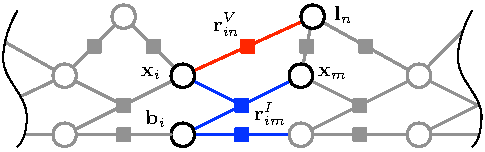
\includegraphics[scale=0.9]{img/graph}
    \caption{A typical fraction of the factor graph, involving state blocks corresponding to keyframes $\bfx_i=(\bfp_i,\bfv_i,\bfR_i)$, biases $\bfb_i$ and landmark poses $\bfl_n$. 
    IMU factors (blue) relate consecutive keyframes and the IMU biases.
    The lower branch controls bias drift along time.
    Visual factors (red) relate landmarks with poses $(\bfp_i,\bfR_i)$.}
    \label{fig:graph}
\end{figure}


\section{Camera extrinsics calibration using Apriltag and kinematics}
\subsection{Motivation}
A camera is placed at an unknown location in a humanoid robot head. We want to estimate the camera pose with respect to the end of the kinematic chain of the robot: the neck joint frame.
The robot's feet are stuck on the ground and we move its torso so that it takes a look around a scene with fixed Apriltags. We want to fuse both kinematic and Apriltag information to estimate the neck camera transformation $\T{K}{C}$.

\subsection{Problem formulation}
The problem is formulated as a factor graph in which keyframes states are poses of a frame from the robot kinematic frame that has a static transform with regard to the camera (the neck joint frame). The camera calibration problem can be expressed as a factor graph represented in figure \ref{fig:factorgraph}. We will estimate simultaneously the neck frame trajectory and the apriltag locations in the scene. As the feet are fixed, we can choose the foot frame as an absolute frame and express both the trajectory and apriltag poses in it.

Then to types of factors constrain the problem.

\subsubsection*{Apriltag factor}
Apriltags are squares landmarks which corner pixel coordinates can be recovered using the Apriltag library. Then given the square width $w$ and the camera model summarized in the intrinsic matrix $\bfK$ (camera images being undistorted), we can recover the relative transformation between the camera frame C and the landmark frame L.
\textit{Conventions}: X-Y-Z = Right-Down-Front for the camera. The landmark frame is chosen so that it has same orientation than the camera frame when the camera is in front of the tag, looking through its center axis.

We have the relation 
\begin{equation}
    \T{W}{L} = \T{W}{B}\T{B}{C}\T{C}{L}
\end{equation}

The state variables of this factor are the landmark and body poses as well as the camera extrinsics $\T{B}{C}$. The measurement we can recover is $\Tm{C}{L}$. Being an element of the Lie group $SE(3)$, the noise on the measurement has to be defined on the local tangent space as explained in \cite{barfoot2017state} so that the sensor model is:

\begin{equation}
    \Tm{C}{L} = \T{C}{L}Exp(\psi) ~~~~ \psi \sim \Gaussian{0}{Q_T}, ~Q_T \in \Reals^{6\times6}
\end{equation}

Then the 6D error function is defined as:

\begin{equation}
    e_{l}(\T{W}{L}, \T{W}{B}, \T{B}{C}) = Log(\T{W}{L} \T{W}{B}^{-1} \T{B}{C}^{-1} \Tm{C}{L}^{-1}) + \psi
\end{equation}

which is a nonlinear function of state variables and measurement with an additive gaussian noise -> we have our factor.

However, we have not determined yet what the measurement covariance $Q_T$ is. Is should somehow be defined according to the pixel noise and the relative pose measurement: the further the landmark is, the greater the uncertainty for instance. A simple yet sensible model for the pixel noise is to assume isotropic and identical gaussian noise on the four pixels recovered. If we stack the four pixels $\bfx_i = [u_i,~v_i]^T \in \Reals^{2}$ in $\bfx = [\bfx_1 ~\bfx_2~ \bfx_3~ \bfx_4]^T$ and define $Q_{\bfx} = \sigma_{\bfx}^2 I_8, ~\sigma_{\bfx} \in \Reals$ being the a pixel noise standard deviation.
A natural way to proceed would be to use the nonlinear covariance propagation scheme using first order approximation.

\begin{equation}
    \begin{split}
        f: \Reals^8 &\rightarrow SE(3) \\
                           \bfx &\rightarrow \T{C}{L} = f_w(\bfx)
    \end{split}
\end{equation}

where the subscript $w$ recalls that each reconstruction depends on the width of the considered tag. 
However, the function f is hard to differentiate since it is an algorithmic process (PnP, ePnP, IPPE...). The function being bijective, we will rather consider its inverse g defined as :

\begin{equation}
    \begin{split}
        g: SE(3) &\rightarrow \Reals^8 \\
                           \T{C}{L} &\rightarrow \bfx = g_w(\T{C}{L})
    \end{split}
\end{equation}


Corners coordinates in the landmark frames can be defined as follows:

\begin{equation}
    c =
    \begin{pmatrix}
    c_1 \\ c_2 \\ c_3 \\ c_4
    \end{pmatrix}
    ~~
    c_1 =  \begin{pmatrix} -1 \\ -1 \\ 0 \end{pmatrix}
    ~ 
    c_2 =  \begin{pmatrix} 1 \\ -1 \\ 0 \end{pmatrix}
    ~
    c_3 =  \begin{pmatrix} 1 \\ 1 \\ 0 \end{pmatrix}
    ~
    c_4 =  \begin{pmatrix} -1 \\ 1 \\ 0 \end{pmatrix}
\end{equation}

where these vectors have been rescaled by a factor $\frac{w}{2}$. This one will be reintroduced later.
Then $\bfx_i = eucl(h_i) = eucl(K\T{C}{L} c_i)$
where $h_i \in \Reals^3$ are the homogenous coordinates associated to the corner projected through the camera lens and $eucl$ represents the "euclideanization" of these coordinates which permits recovering corresponding pixel coordinates. 

\begin{equation}
    \begin{split}
        eucl: \Reals^3 &\rightarrow \Reals^2 \\
                           h = \begin{pmatrix}x\\y\\z\end{pmatrix} &\rightarrow \bfx = \begin{pmatrix}x/z\\y/z\end{pmatrix}
    \end{split}
\end{equation}


We need to compute the jacobian for each corner pixel variation $J^{x_i}_{\T{C}{L}} = J^{x_i}_{h_i} J^{h_i}_{\T{C}{L}} $ (chain rule) where the first jacobian corresponds to the euclideanization and the second the projection to homogeneous coordinates.

Regardind the jacobian with respect to the $SE(3)$ element, we will instead choose to consider the transformation as an element of $SO(3)\times T(3)$ since this is the way poses are treated in Ceres. The projection function and its jacobians with respect to the measured translation and rotation then write:

\begin{equation}
\begin{split}
    &h_i = K(\Rot{C}{L}c_i + \prescript{C}{}{t}_L) \\
    &J^{h_i}_{\prescript{C}{}{t}_L} = K ~~~~~~ J^{h_i}_{\Rot{C}{L}} = -K\Rot{C}{L}[c_i]_{\times}  ~~~~~~  J^{h_i}_{\T{C}{L}} = [J^{h_i}_{\prescript{C}{}{t}_L} ~J^{h_i}_{\Rot{C}{L}}]
\end{split}
\end{equation}

The euclideanization jacobian is found to be:

\begin{equation}
    J^{x_i}_{h_i}
    =
    \begin{pmatrix}
    1/z_i & 0 & -x_i/z_i^2 \\
    0 & 1/z_i & -y_i/z_i^2
    \end{pmatrix}
\end{equation}

Finally, we can stack the 4 jacobians to get the full jacobian to be used for covariance propagation.

\begin{equation}
    J \triangleq J^{\bfx}_{\T{C}{L}}=
    \frac{w}{2}
    \begin{pmatrix}
    J^{\bfx_1}_{\T{C}{L}} \\ J^{\bfx_2}_{\T{C}{L}} \\ J^{\bfx_3}_{\T{C}{L}} \\ J^{\bfx_4}_{\T{C}{L}}
    \end{pmatrix}
    ~ \in \Reals^{8 \times 6}
\end{equation}
reintroduction the $\frac{w}{2}$ factor common to the 4 corners. 

We therefore have the covariance propagation equation $Q_{\bfx} = J Q_{\T{C}{L}} J^T$. This equation must be inverted in order to recover the needed covariance. $J$ being non square, we have to use the pseudo inverse to write: $Q_{\T{C}{L}} = pinv(J^T) Q_{\bfx} pinv(J)$. Knowing that the pixel noise covariance is isotropic as explained above, this equation simplifies to:

\begin{equation}
Q_{\T{C}{L}} = \sigma_{\bfx}^2(J^T J)^{-1}    
\end{equation}





\subsubsection*{Kinematic unary factor (Wolf Pose3D)}
6D unary factor constraining the ith keyframe pose:

\begin{equation*}
e(\T{F}{K_i}) = Log_{SE(3)}(\Tm{F}{K_i}^{-1} \T{F}{K_i})    
\end{equation*}



\section{Kinematic odometry}
The goal of this section is to find a way to use kinematics measurements of the pose of the body frame relative to its contacts with the environment as well as feet force torque sensors to design a relative pose factor (Odom3D in wolf jargon) between body frames at different timestamp. Force torque sensors will be used as a way to determine the contact states, that is to say whether or not the contact remains static from one timestamp to an other: for example a support foot could be slipping on the ground, tilting on an edge etc.
Special care will be given to the computation of the different measurements covariances that depend on the contact states, kinematic inconsistencies or flexibilities, encoders errors...

\subsection{Odom3D factor}
An 3D odometry factor constraints two poses through a relative pose measurement. In our case the, poses we which to constraints are the absolute pose of the body frame from timestamps $t_{i-1}$ and $t_{i}$: $\T{W}{B_{i-1}}$ and $\T{W}{B_i}$. The residual of this factor is defined as $\bfr^2 = ||\bfe(\T{W}{B_{i-1}}, \T{W}{B_i})||^2_{\bfQ_{i/i-1}}$
 with:
 
 \begin{equation*}
 \bfe(\T{W}{B_{i-1}}, \T{W}{B_i}) =  Log_{SE(3)}(
 \T{W}{B_{i-1}}^{-1}
 \T{W}{B_i}
 \T{B_{i-1}}{B_i}^{-1}
 )     
 \end{equation*} 

\subsection{Single foot in support phase}
Let's begin with a simplified case of a humanoid robot in support phase on a single foot.
We want to measure the relative pose of the base frame at times $t_{i-1}$ and $t_i$. This pose can be decomposed in three poses: 

\begin{equation*}
\Tm{B_{i-1}}{B_i} = 
\Tm{B_{i-1}}{F_{i-1}}
\Tm{F_{i-1}}{F_{i}} 
\Tm{F_{i}}{B_i}     
\end{equation*}

A few comments on the different quantities. $ \Tm{B_{i-1}}{F_{i-1}} $ and $ \Tm{F_{i}}{B_i} $ are kinematic measurements made at time $t_{i-1}$ and $t_{i}$ respectively that are affected by the encoder noises, kinematic model inconsistencies and robot flexibilities (TODO). However, we have no direct measurement over $\Tm{F_{i-1}}{F_{i}}$. One way to proceed is to assume that $\Tm{F_{i-1}}{F_{i}}=\bfI_4$ and assign it a covariance based on the foot force/torque sensors measurements (TODO inspired by Thomas F.). Then these three measurements are composed to get a covariance on $\Tm{B_{i-1}}{B_i}$ using first order approximation or as explained in \cite{barfoot2014associating}.

\subsection{Fusing multiple contacts}
In the case of humanoid locomotion we have 2 pose measurements of the same quantity using both foot. 

One easier way to implement it is to include both measurements as separate Odom3D factors in the graph. Measurements with covariance too high (foot flying, slipping or tilting) can be plainly discarded using an upper threshold on the covariance determinant.

Another option is to fuse in an optimal way the pose measurements based on there covariances. This would result in a single factor and is the problem tackled in section IV of \cite{barfoot2014associating}. This enables handling an arbitrary number of contacts with reduced computational burden.


\section{Center of mass estimation}
\subsection{Motivation}
In this section we want to derive factors in order to observe inertial quantities of the robot, that is to say its center of mass (COM), center of mass velocity and angular momentum (AM). Many papers have addressed this issue by fusing kinematic and force torque measurements.
Biblio:
- Stephens
- Xinjilefu
- Bloesch
- Bloesch student
- Carpentier/Bailly
- Bae

The common elements of most of these work is that they are decoupled from the estimation of base quantities of the robot (position, velocity, orientation) except for Bae et al. (more biblio needed to confirm). Here we propose to assess the possibility and the possible improvements of considering a more tightly coupled approach, designing a single tightly coupled estimator reconstructing all quantities by solving a nonlinear optimization problem as explained in eq \ref{eq:leastsquare}. The considered quantities are stacked in the state vector: 

\begin{equation*}
\bfx = [\posi{W}{WB}, \vel{W}{WB}, \Rot{W}{B}, \posi{W}{WC}, \vel{W}{WC}, \prescript{W}{}{\AM}_{c}] 
\triangleq 
[\bfp, \bfv, \Rot{}{}, \COM, \COMd, \AM_c] 
\end{equation*}

where $B$ and $C$ correspond to the frame/frame origin (appropriately) of the robot body and the COM. Notations of the state blocks are simplified in order to make it easier to differentiate them with other terms in the subsequent equations.

It is assumed that there are enough factors in the problem to make the base quantities observable (Apriltag + IMU factors). We need to define factors constraining the inertial quantities with the other ones in order to make the whole system observable. For this we have access to different sources information.
\begin{enumerate}
    \item Force/Torque sensors: placed at the end effectors of the robot, these give us measurements of the contact wrench expressed at the sensor location and in the local frame. 
    \item Kinematic measurements: based on the inertial kinematic model of the robot, we can retrieve relative transformations and velocities between robot frames as well as a direct measurement of the COM position and velocities relative to the base.
    \item Base angular velocity: Usually coming from an IMU, we could also consider using angular velocity measurements coming from the robot kinematics
\end{enumerate}

We will develop 2 factors: 

\begin{itemize}
    \item An inertial kinematics factor relating inertial quantities with base ones at a given time
    \item A preintegrated Force/Torque factor combining several successive F/T measurements as well as kinematics quantities to constrain states at distant intervals (freq $\sim$ FTfreq/200)
\end{itemize}


\subsection{Inertial kinematics}
\subsubsection{Vectorial equations}
It is possible to derive equations relating instantaneous relations between inertial quantities and the body quantities through kinematics considerations.
First, the velocity composition law on the COM between the world and body frame writes in vectorial form:
\begin{equation}
\dot{\COMv} = \velv{B} + \angvelv{B} \times \posiv{BC}(q_A) + \velv{BC}(q,\dot{q}) 
\end{equation}

The angular momentum of a multibody system can be decomposed in two terms as follows.

\begin{equation}
\AMv_c = \bfI(q_A) \angvelv{B} + \AMv_q (q,\dot{q})   
\end{equation}

where

\begin{itemize}
    \item \( \angvel{}{B} \): angular velocity vector describing the rotation rate of frame B with respect to the observer inertial frame
    \item \( \bfI(q_A) \): inertia matrix of the robot expressed at the COM
    \item \( \AM_q (q,\dot{q}) \): Angular momentum of the limbs ("gesticulation")
\end{itemize}

\textbf{HYP}: the inertia matrix and gesticulation terms are perfectly known: they don't enter the system as measurements but as "parameters". This could be relaxed once it is tested in simulation.

Also very simply, the COM position (in the world frame) can be transformed from its position in body frame:

\begin{equation}
    \COM = \Rot{}{} \posi{B}{BC}(q_A) + \posi{}{}
\end{equation}

\subsubsection{Sensor model}
Great care should be given defining a measurement model for \(\posi{B}{BC}(q_A)\). This data is potentially corrupted by 3 factors:

\begin{itemize}
    \item encoder noise
    \item errors in the inertial/kinematic model of the robot
    \item structural flexibilities
\end{itemize}

While the first term could be regarded as a Gaussian perturbation, the two others are clearly bias terms that depend strongly on robot configuration and the dynamics/phases of the movement.  
We will consider the quantity $\posi{b}{BC}$  as a measurement disturbed by a Gaussian noise and a time varying bias considered constant during pre-integration period.

\begin{equation}
\posim{B}{BC} = \posi{B}{BC}(q_A) + \bias_{p} + \noise_p 
\end{equation}


All other terms computed through direct kinematics are in first hand considered as exact values but are in fact corrupted by (supposedly) gaussian noise due to encoder noise, flexibilities, model errors...

\begin{equation}
\begin{split}
\posim{A}{AB} = \posi{A}{AB}(q_A) + \noise_p ~~~ \noise_p \sim \Gaussian{0}{Q_p}, ~ Q_p \in \Reals^{3\times 3} 
\\
\velm{A}{AB} = \vel{A}{AB}(q_A) + \noise_v ~~~ \noise_v \sim \Gaussian{0}{Q_v}, ~ Q_v \in \Reals^{3\times 3} 
\\
\Rotm{A}{B} = \Rot{A}{B}(q_A) Exp(\phi) ~~~ \phi \sim \Gaussian{0}{Q_{\phi}}, ~ Q_{\phi} \in \Reals^{3\times 3}
\end{split}
\end{equation}
 
An \textbf{important} thing to take into account is the fact that some of the kinematic measurement noise can be correlated. For instance the relative position shoulder-hand is strongly correlated with the shoulder-elbow one. Some others are less obvious (hand velocity/hand position?). As for the relative poses measurements, one way to deal with these hard to model correlations is to decompose the measurements so that the noise random variables can be reasonably considered independent. One idea is to consider (if such exists) a root frame by which the considered kinematic chain is passing.

\subsubsection{Factor formulation}

Given the previously explained measurement models of $\angvel{B}{WB}$ and $\posi{B}{BC}$, we can project these equations in the world frame. We also add a relation between the COM position expressed in the world frame and its body frame relative measurement:

\begin{equation}
\begin{split}
\COM &= \Rot{}{} (\posim{B}{BC} -  \bias_{p} - \noise_p) + \posi{}{}
\\
\COMd &= \vel{}{} + \Rot{}{}((\angvelm{B}{B} - \bias_{\omega} - \noise_{\omega}) \times (\posim{B}{BC} -  \bias_{p} - \noise_p) + (\velm{B}{BC} - \noise_v))
\\
\AM_c &= \Rot{}{}(\bfI(q_A) (\angvelm{B}{B} - \bias_{\omega} - \noise_{\omega}) + \AM_q (q,\dot{q}))
\end{split}
\end{equation}

Given these equations, we will now define error random variables as a function of the states and their related covariance matrix. The direct kinematics is easy to put in the form $y = h(x) + n$ and therefore the error function is simply  $e(x) = y - h(x) ~~~ e \sim \Gaussian{0}{Q_n}$. 

\begin{equation}
\begin{split}
\bfe_{ikin}(\posi{}{}, \Rot{}{}, \vel{}{}, \COM, \COMd, \AM_c, \bias_p, \bias_{\omega}, \noise_p, \noise_v, \noise_{\omega}) &= 
\begin{pmatrix}
\bfe_{\COM}(\COM, \posi{}{}, \Rot{}{}, \noise_p)
\\
\bfe_{\COMd}(\COMd, \vel{}{}, \Rot{}{}, \bias_{\omega}, \bias_p, \noise_p, \noise_v, \noise_{\omega})
\\
\bfe_{\AM_c}(\AM_c, \Rotm{}{}, \bias_{\omega}, \noise_{\omega})
\end{pmatrix}
\\
&=
\begin{pmatrix}
\posim{B}{BC} + \noise_p - (\Rot{}{}^T(\COM - \posi{}{}) + \bias_{p})
\\
(\angvelm{B}{B} - \bias_{\omega} - \noise_{\omega}) \times (\posim{B}{BC} -  \bias_{p} - \noise_p) + \velm{B}{BC} - \noise_v - \Rot{}{}^T(\COMd - \vel{}{})
\\
\bfI(q_A) (\angvelm{B}{B} - \bias_{\omega} - \noise_{\omega}) + \AM_q (q,\dot{q}) - \Rot{}{}^T\AM_c
\end{pmatrix}
\end{split}
\end{equation}

The second requires linearization with regard to the biases $\noise_{\omega}$ and $\noise_{p}$ in order to get its covariance matrix. Keeping the noise terms:

\begin{equation}
    \bfe_{\COMd} = cst(\noise_{\omega}, \noise_{p}, \noise_{v}) - [\angvelm{B}{B} - \bias_{\omega}]_{\times}\noise_p + [\posim{B}{BC} -  \bias_{p}]_{\times}\noise_{\omega} - \noise_v + \noise_{\omega}\times\noise_p
\end{equation}

Neglecting the last nonlinear term in the $\COMd$ equation, we thus have a linear relation between measurement noises and error functions. 
Noting $\bfe_n$ the noisy error (random variable), we can derive the linear transformation from $\bfe_n$ with respect to the noise vector $\noise_{ikin} = (\noise_p^T, \noise_v^T, \noise_{\omega}^T)^T$.

\begin{equation}
\bfJ^{\bfe}_{\noise} = 
\begin{pmatrix}
\Ident & 0 & 0 
\\
- [\angvelm{B}{B} - \bias_{\omega}]_{\times} & -\Ident & [\posim{B}{BC} -  \bias_{p}]_{\times}
\\
0 & 0 & -\bfI(q_A)
\end{pmatrix}
\end{equation}

Then the covariance matrix associated to the error vector is $Q_e = \bfJ^{\bfe_{ikin}}_{\noise_{ikin}} Q_{\noise_{ikin}} \bfJ^{\bfe_{ikin} T}_{\noise_{ikin}}$ and the residual passed to the solver is $r_{ikin} = Q_{\bfe_{ikin}}^{-1/2} \bfe_{ikin}$.

Defining $\bar{\angvel{}{}} = \angvelm{}{} - \bias_{\angvel{}{}}$,  $\bar{p} = \posim{B}{BC} - \bias_p$, the covariance structure is:

\begin{equation}
Q_{ikin} = 
\begin{pmatrix}
Q_p  &  Q_p[\bar{\omega}]_{\times} & 0
\\
-[\bar{\omega}]_{\times}Q_p & Q_{pv\omega}& -[\bar{p}]_{\times}Q_{\omega}\bfI(q_A)
\\
0 & -Q_{\omega}\bfI(q_A)[\bar{p}]_{\times} & \bfI(q_A)Q_{\omega}\bfI(q_A)
\end{pmatrix}
\end{equation}

where $Q_{pv\omega} = -[\bar{\omega}]_{\times}Q_p[\bar{\omega}]_{\times} + Q_v - [\bar{p}]_{\times}Q_{\omega}[\bar{p}]_{\times} $.

One thing to note is that the jacobian depends on the current bias estimates. Either the bias at the factor creation should be used hence the jacobian is constant and does not have to be recomputed or we recompute the covariance matrix each time a new bias estimate is available.


\subsection{Force/torque sensors factor}
A relation between these quantities will be derived through the Newton-Euler equations. It will be shown that by expressing these equation at the COM a chosen inertial frame $W$, as it is usually done, the position velocity and orientation appear naturally in the equations.
With this formulation, the factor will also include a base angular velocity measurements source, usually coming from the IMU or differential kinematics.

\textit{Notation note}: The robot is considered to possess N limbs equipped with 6D wrench sensors which measurements will be indexed by the lowercase $l$. We will denote by $L$ the sensor frame associated with limb $l$.

\subsubsection{Vectorial equations}
The Newton-Euler equations at the COM with respect to an inertial frame can be written:

\begin{equation}
\begin{split}
m\ddot{\COMv}&= m\gravv + \sum_l \forcev{l}
\\
\dot{\AMv}_c&= \sum_l \torquev{l} + ( \posiv{L} - \COMv) \times \forcev{l} 
\end{split}
\label{eq:NewtonEuler}
\end{equation}

where \(\posiv{L} \) is the position vector of each end effector in the inertial frame.

\subsubsection{Force/torque sensors measurements model}

Each end effector $l \in 1..N$ is equipped with a sensor measuring forces $\bff \in \Reals^3$ and pure torques $\tau \in \Reals^3$ along the three orthogonal axis of its reference frame. The measurements are assumed to be corrupted by a zero mean Gaussian noise:

\begin{equation}
\begin{split}
    \forcem{}{l} = \force{L}{l} + \noise_f~~~~~\noise_f \sim \mathcal{N}(O,Q_{\bff})
    \\
    \torquem{}{l} = \torque{L}{l} + \noise_{\tau} ~~~~~ \noise_{\tau} \sim \mathcal{N}(O,Q_{\tau})
\end{split}
\end{equation} 
for $l \in 1..N$, with N number of force sensors and L the frame attached to this sensor (that we will drop subsequently for shorter notations).

\textbf{Unknown biases} drifting with time could potentially be added and estimated (TBD). 
In all equations, unless otherwise specified kinematic measurements (depending on $q$ and $\dot{q}$) are considered to be exact. We should consider adding them in the measurement vector in a second time to account for encoder noises or flexibilities.
For lighter notation we will subsequently omit the measurement frame of references noting simply \(\forcem{}{l}\) and \(\torquem{}{l}\) for force and torque measurement values.

When equations are discretized, the measurements recovered at time $t_k$ permit to deduce state at time $t_k$ given $t_{k-1}$. In this factor, we will consider uncertainties only on the N force torque sensors and bias + noise on the relative COM position measurement. The raw measurement vector for N limbs is therefore:

\begin{equation}
z_k = \left[ \left[\forcem{}{l}^k \right]_{l \in [1..N}, \left[\torquem{}{l}^k \right]_{l \in [1..N}, \posim{}{BC}^k \right]
\end{equation}
%

Incorporation of kinematic information is done through exact recovery of relative position and rotations using the articulary configuration of the robot $q_A$ and its kinematics model. In the discrete case, we simplify the notation using only the $k$ subscript, writing for instance $\posi{B}{BL}^k$ instead of $\posi{B}{BL}(q_A^k)$.

\subsubsection{Factor formulation}
Incorporating the measurements model in equation \ref{eq:NewtonEuler} and expressing it in the world frame \(W\), we derive the equations:

\begin{equation}
\begin{split}
m\ddot{\COM}&= 
m\bfg + \Rot{}{} \sum_l \Rot{B}{L}(q_A) (\forcem{}{l} - \noise_f) 
\\
\dot{\AM}_c&= 
\sum_l \Rot{}{}\Rot{B}{L}(q_A)(\torquem{}{l} - \noise_{\tau}) + (\Rot{}{} \posi{B}{CL}(q_A)) \times (\Rot{}{}\Rot{B}{L}(q_A)(\forcem{}{l} - \noise_f))
\\
&= \sum_l \Rot{}{}\Rot{B}{L}(q_A)(\torquem{}{l} - \noise_{\tau}) + \Rot{}{}( \posi{B}{BL}(q_A) - (\posim{B}{BC}(q_A)) -  \bias_{p} - \noise_p) \times (\Rot{B}{L}(q_A)(\forcem{}{l} - \noise_f))
\end{split}
\end{equation}

It can be reformulated as the state-space model equation on the COM related variables \( \frac{d\bfx_c}{dt}= f(\bfx_c, \bfu, t)$ with $\bfx_c = [\COM, \COMd, \AM_c]\):

\begin{equation}
\begin{split}
\frac{d\COM}{dt} &= \COMd 
\\
\frac{d\dot{\bfc}}{dt}&= \bfg + \frac{1}{m} \Rot{}{} \sum_l \Rot{B}{L}(q_A) (\forcem{}{l} - \noise_f) 
\\
\frac{d\AM_c}{dt}&= \Rot{}{} \sum_l \Rot{B}{L}(q_A)(\torquem{}{l} - \noise_{\tau}) + (\posi{B}{BL}(q_A) - (\posim{B}{BC}(q_A)) -  \bias_{p} - \noise_p) \times (\Rot{B}{L}(q_A)(\forcem{}{l} - \noise_f))
\end{split}
\label{eq:COMContinuous}
\end{equation}


We now need to discretize this continuous system to define factors between successive times. We integrate \ref{eq:COMContinuous} between 2 consecutive measurements ($t_k$ and $t_{k+1}$ $\delta t = t_{k} - t_{k-1}$)  We use a simple first order approximation (forward Euler) which consists in assuming a zero order hold on measurements. We may also add a second order term for the com position since we have measurements on its acceleration.

\begin{equation}
\begin{split}
\COM^{k} &= \COM^{k-1} + \COMd^{k-1} \delta t 
+ \frac{1}{2} \bfg \delta t^2 + \frac{1}{2m} \Rot{}{}^{k-1} \sum_l \Rot{B}{L}^{k} (\forcem{}{l}^{k} - \noise_f^{k}) \delta t^2
\\
\COMd^{k}&= \COMd^{k-1} + \bfg \delta t + \frac{1}{m} \Rot{}{}^{k} \sum_l \Rot{B}{L}^{k} (\forcem{}{l}^{k} - \noise_f^{k}) \delta t 
\\
\AM_c^{k} &= \AM_c^{k-1} +  ( 
\Rot{}{}^{k}\sum_l \Rot{B}{L}^{k}(\torquem{}{l}^{k} - \noise_{\tau}^{k}) + (\posi{B}{BL}^{k} - \posim{B}{BC}^{k} + \bias_{p}^{k} + \noise_p^{k}) \times \Rot{B}{L}^{k}(\forcem{}{l}^{k} - \noise_f^{k}) 
) \delta t
\end{split}
\label{eq:COMDiscrete}
\end{equation}

with discrete noise quantities distributed according to \( \mathcal{N}(O,\frac{Q}{\delta t}) \), \(Q\) being the corresponding continuous covariance.

\paragraph{Adding kinematic noise}

If we consider kinematic measurements to be noisy, have to write that:

\begin{equation}
	\begin{split}
	\Rotm{B}{L} &= \Rot{B}{L} Exp(\delta \phi_{BL}) \simeq \Rot{B}{L} (I + [\delta \phi_{BL}]_{\times})
	\\
	\posim{B}{BL} &= \posi{B}{BL} + \delta p_{BL}
	\end{split}
\end{equation}

Then eqs \ref{eq:COMDiscrete} write:



\begin{small}
\begin{equation}
\begin{split}
\COM^{k} &= \COM^{k-1} + \COMd^{k-1} \delta t 
+ \frac{1}{2} \bfg \delta t^2 + \frac{1}{2m} \Rot{}{}^{k-1} \sum_l \Rotm{B}{L}^k (I - [\delta \phi_{BL}]_{\times}^{k}) (\forcem{}{l}^{k} - \noise_f^{k}) \delta t^2
\\
\COMd^{k}&= \COMd^{k-1} + \bfg \delta t + \frac{1}{m} \Rot{}{}^{k} \sum_l \Rotm{B}{L}^k (I - [\delta \phi_{BL}]_{\times}) (\forcem{}{l}^{k} - \noise_f^{k}) \delta t 
\\
\AM_c^{k} &= \AM_c^{k-1} +  ( 
\Rot{}{}^{k}\sum_l \Rotm{B}{L}^k (I - [\delta \phi_{BL}]_{\times}) (\torquem{}{l}^{k} - \noise_{\tau}^{k}) + (\posi{B}{BL} - \delta p_{BL} - \posim{B}{BC}^{k} + \bias_{p}^{k} + \noise_p^{k}) \times \Rotm{B}{L}^k (I - [\delta \phi_{BL}^k]_{\times}) (\forcem{}{l}^{k} - \noise_f^{k}) 
) \delta t
\end{split}
\label{eq:COMDiscrete}
\end{equation}
\end{small}

We will first derive equations without noisy measurements and then, with them.

\subsubsection{Factor between successive measurements}
Rearranging the terms of eq \ref{eq:COMDiscrete}, we can express the relationships as measurement functions $\bfy = h_{FT}(\bfx) + \noise_y$ with $\bfy$ and $\noise_{\bfy}$ depending only on bias term $\bfp$:

\begin{small}
\begin{equation}
\begin{split}
	\frac{1}{2m}\sum_l \Rot{B}{L}^{k} \forcem{}{l}^{k}\delta t^2 =& 
	\Rot{}{}^{k-1,T}(\COM^{k} - \COM^{k-1} - \COMd^{k-1} \delta t - \frac{1}{2} \bfg \delta t^2)
	+ \frac{1}{2m}\sum_l \Rot{B}{L}^{k} \noise_f^{k}\delta t^2
	\\
	\frac{1}{m} \sum_l \Rot{B}{L}^{k} \forcem{}{l}^{k} \delta t =& \Rot{}{}^{k-1,T}(\COMd^{k} - \COMd^{k-1} - \bfg \delta t) 
	+ \frac{1}{m} \sum_l \Rot{B}{L}^{k} \noise_f^{k} \delta t	
\end{split}
\label{eq:CCdFactor}
\end{equation}
\end{small}

\begin{small}
\begin{equation}
\begin{split}
	(\sum_l \Rot{B}{L}^{k}\torquem{}{l}^{k} + (\posi{B}{BL}^{k} - \posim{B}{BC}^{k} + \bias_{p}^{k-1}) \times \Rot{B}{L}^{k}\forcem{}{l}^{k}) \delta t = 
	\Rot{}{}^{k-1,T}(\AM_c^{k} - \AM_c^{k-1})
	\\
	+ (\sum_l \Rot{B}{L}^{k}\noise_{\tau}^{k} + (\posi{B}{BL}^{k} - \posim{B}{BC}^{k} + \bias_{p}^{k})\times \Rot{B}{L}^{k}\noise_f^{k}  + \Rot{B}{L}^{k}\forcem{}{l}^{k}  \times \noise_p^{k} + \noise^k_p \times \noise^k_f)\delta t
\end{split}
\label{eq:LcFactor}
\end{equation}
\end{small}

\begin{equation}
\bfy_{FT} =
\begin{pmatrix}
y_{\COM} \\ y_{\COMd} \\ y_{\AM}(\bias_{p}^{k-1})
\end{pmatrix}
=
\begin{pmatrix}
h_{\COM}(\COM^{k}, \COM^{k-1}, \COMd^{k}, \Rot{}{}^{k-1})
\\
h_{\COMd}(\COMd^{k}, \COMd^{k-1}, \Rot{}{}^{k-1}) 
\\
h_{\AM}(\AM_c^{k}, \AM_c^{k-1}, \Rot{}{}^{k-1})
\end{pmatrix}
+
\begin{pmatrix}
\noise_{\COM}(\noise_f^{k})
\\
\noise_{\COMd}(\noise_f^{k})
\\
\noise_{\AM}(\bias_{p}^k, \noise_p^k, \noise_f^{k}, \noise_\tau^{k})
\end{pmatrix}
\end{equation}

Then, to get the covariance matrix of $\noise_y$, we have to recover the linear relation $\noise_y = J^{\noise_y}_{\noise_z}$ from eqs \ref{eq:CCdFactor} and \ref{eq:LcFactor}.

Neglecting the nonlinear term $\noise_p \times \noise_f$ in eq \ref{eq:LcFactor}, we get (for N=2 limbs):

\begin{equation}
	J^{\noise_y}_{\noise_z} =
	\begin{pmatrix}
    \Rot{B}{L_1}^k \delta t^2/2m & \Rot{B}{L_2}^k \delta t^2/2m & 0 & 0 & 0 
    \\
    \Rot{B}{L_1}^k \delta t/m & \Rot{B}{L_2}^k \delta t/m & 0 & 0 & 0 
    \\
    \left[(\posim{B}{BL_1}^k - \posibar_{BC}^k) \right]_{\times} \Rot{B}{L_1}^k \delta t & \left[(\posim{B}{BL_2}^k - \posibar_{BC}^k) \right]_{\times} \Rot{B}{L_2}^k \delta t & \Rot{B}{L_1}^k \delta t & \Rot{B}{L_2}^k \delta t & \sum_l [\Rotm{B}{L}^k \forcem{}{l}^k]_{\times} \delta t
	\end{pmatrix}
\end{equation}

Then $Q_{\noise_{FT}} = J^{\noise_{FT}}_{\noise_{ft}} Q_{\noise_{ft}} J^{\noise_{FT},T}_{\noise_{ft}}$. Note that the jacobian depends on the bias variable and that therefore the covariance should be recomputed at each new solve of the problem.

However this formulation requires to create new variables (Key Frames) at the measurement frequency which quickly becomes intractable if the older states are not marginalized (windowed optimization). However, a mathematical trick enables to preintegrate consecutive measurements to create factors between distant (Lupton \cite{lupton2011visual}/Forster's \cite{forster2016manifold} preintegration).  

\subsubsection{Pre-integrated COM factor}
This section is very much inspired by the structure, developments and notations of \cite{forster2016manifold}.
Adding measurements between 2 arbitrary timestamps \(t_i\) and \(t_j\) with \(\Delta t_{ij} \triangleq t_j - t_i\), we get the equations:

\begin{equation}
\begin{split}
\COM^{k} - \COM^{i} &= \sum_{j=i+1}^{k} \Big[ 
\COMd^{j-1} \delta t 
+ \frac{1}{2}\bfg \Delta t^2 + \frac{1}{2m} \Rot{}{}^{j-1} \sum_l \Rot{B}{L}(q^{j}) (\forcem{}{l}^{j} - \noise_f^{j})\Delta t^2 \Big]
\\
\COMd^{k} - \COMd^{i} &= \sum_{j=i+1}^{k} \Big[ 
\bfg + \frac{1}{m} \Rot{}{}^{j} \sum_l \Rot{B}{L}(q^{j}) (\forcem{}{l}^{j} - \noise_f^{j}) \Big] \delta t 
\\
\AM_c^{k} - \AM_c^{i} &=  \sum_{j=i+1}^{k} \Rot{}{}^{j} \Big[ 
\sum_l \Rot{B}{L}(q^{j-1}) (\torquem{}{l}^{j} - \noise_{\tau}^{j}) - (\forcem{}{l}^{j} - \noise_f^{j}) \times (\posi{B}{BL}(q^j) - \posim{B}{BC}^j + \bias_{p}^j + \noise_p^j) \Big]  \Delta t
\end{split}
\label{eq:COMij}
\end{equation}

An important assumption to be made in order to keep the efficiency of the method is to consider that biases terms (angular velocity and relative position) as constant during the preintegration period, that is to say $\forall j \in [i..k-1], \bias_p^j = \bias_p^i $. Therefore, each keyframe is composed of the usual state variables (described earlier) and estimated bias terms considered constant until the next keyframe. This prevents the explosion of state variable number as well as permits to easily debias the preintegrated measurements through first order linearization. We will come back to validity warnings about this method later.
It is then possible to define a "delta" quantity depending only on the measurements relating the com position, com velocity and Angular Momentum at \(t_i\) and \(t_j\):

\begin{equation}
\begin{split}
    \Delta \COM_{ik} &\triangleq \Rot{}{}^{i,T} (\COM^k - \COM^i - \COMd{}{}^i \Delta t_{ik} - \frac{1}{2}\grav \Delta t_{ik}^2) 
    \\
    &= \sum_{j=i+1}^{k} \Big[ \Delta \COMd_{ij} \delta t + \frac{1}{2m} \Delta R_{ij} \sum_l \Rot{B}{L}(q^{j}) (\forcem{}{l}^{j} - \noise_f^{j}) \Delta t^2 \Big]
\\
    \Delta \COMd_{ik} &\triangleq \Rot{}{}^{i,T} (\COMd^{k} - \COMd^{i} - \bfg \Delta t_{ik})
\\
    &= \frac{1}{m} \sum_{j=i+1}^{k} \Delta R_{ij} \sum_l \Rot{B}{L}(q^{j}) (\forcem{}{l}^{j} - \noise_f^{j}) \delta t 
\\
    \Delta \AM_{ik} &\triangleq \Rot{}{}^{i,T} (\AM_c^{k} - \AM_c^{i})
\\
     &=  \sum_{j=i+1}^{k} \Delta R_{ij} \Big[ 
    \sum_l \Rot{B}{L}(q^{j}) (\torquem{}{l}^{j} - \noise_{\tau}^{j} - (\forcem{}{l}^{j} - \noise_f^{j}) \times (\posi{B}{BL}(q^j) - \posim{B}{BC}^j + \bias_{p}^i + \noise_p^j)) \Big]  \Delta t
\end{split}
\label{eq:DeltaFT}
\end{equation}

where the $\Delta \Rot{}{ij}$ comes from preintegration of the angular velocity measurements which constraints orientation of the base at times $t_i$ and $t_k$.

\begin{equation}
    \Delta \Rot{}{ik} = \Rot{}{i}^T \Rot{}{k}
    = \prod_{j=i+1}^{k} Exp((\angvelm{}{}^j - \bias_{\omega}^i - \noise_{\omega}^j)\Delta t)
    \label{eq:DeltaR}
\end{equation}

The question is whether or not to include it in the inertial factor. If we want to take into account the between the different quantities due to the angular velocity measurements, we have to include it. In this case the factor is 12 dimension and the covariance has to be propagated accordingly.


We can then define a recursive scheme to retrieve measurement values and a covariance propagation scheme akin to the IMU pre-integration framework. 
Difficulties that might come up during implementation:

\begin{itemize}
    \item Angular velocity and force/torque measurements are not recovered at the same frequency -> consider a constant delta for the slowest one?
    \item COM preint factor noise is correlated with the IMU one since the gyro noise is propagated through it as well.
\end{itemize}

We will thereafter consider the 2 difficulties as hypothesis: 
\\
- angular velocity and force/torque sensor sources are at the same frequency. 
\\
- we have to add the rotation part to the inertial kinematic residual in order to have a properly formulated factor. To recover the 9D residual and 9x9 covariance matrix, these just have to be extracted from the full 12D residual and 12x12 covariance matrix that we will derive thereafter.


Equations \ref{eq:DeltaFT} and \ref{eq:DeltaR} relate state variables at time i and j (left hand side) to the measurements (right hand side). However, since the noise terms are quite intrically spread in the equations, they require more treatment in order to be able to use them to define error functions and covariance of the factor. In order to do that, we will consider a first order approximation in noise terms in order. First, let us consider the $\Delta R_{ik}$ equation \ref{eq:DeltaR}:

\begin{equation}
\begin{split}
\Delta \Rot{}{ik} &\simeq  \prod_{j=i+1}^{k} Exp(\angvelm{}{}^j - \bias_{\omega}^i) Exp(-J^j_r \noise_{\omega}^j\Delta t)
\\
&= \Delta \Rotm{}{ik}\prod_{j=i}^{k-1} Exp(- \Delta \Rotm{}{ij+1} J^j_r \noise_{\omega}^j\Delta t)
\\
&= \Delta \Rotm{}{ik}Exp(-\delta \phi_{ik})
\end{split}
\end{equation}

where $J^k_r \triangleq J_r((\angvelm{}{}^k - \bias_{\omega}^i))\Delta t)$ is the right exponential jacobian, the preintegation rotation measurement is defined as 
\begin{equation}
    \Delta \Rotm{}{ik} \triangleq \prod_{j=i}^{k-1} Exp(\angvelm{}{}^j - \bias_{\omega}^i)
\end{equation}
and the noise term $\delta \phi_{ik}$ will be detailed later. Note that the second inequality comes from the SO(3) exponential useful property that $ Exp(\phi)\Rot{}{} = \Rot{}{} Exp(\Rot{}{}^T \phi)$ applied recursively (with $\Delta \Rotm{}{ij+1}$ terms appearing inside the noise exponential).

Then we can treat the relative com velocity equation by using the first order matrix exponential approximation $Exp(\phi) \simeq \Ident + [\phi]_{\times}$:

\begin{equation}
\begin{split}
\Delta \COMd_{ik} &\simeq
\frac{1}{m} \sum_{j=i+1}^{k} \Delta \Rotm{}{ij}(\Ident - [\phi_{ij}]_{\times}) \sum_l \Rot{B}{L}(q^{j}) (\forcem{}{l}^{j} - \noise_f^{j}) \delta t 
\\
&= \Delta \COMdm_{ik} + \frac{1}{m} \sum_{j=i+1}^{k} \Delta \Rotm{}{ij}[\phi_{ij}]_{\times} \sum_l \Rot{B}{L}(q^{j})\noise_f^{j} \Delta t
\\
&= \Delta \COMdm_{ik} - \delta \COMd_{ik}
\end{split}
\end{equation}

where the delta measurement is defined as
\begin{equation}
    \Delta \COMdm_{ik} \triangleq \frac{1}{m} \sum_{j=i+1}^{k} \Delta \Rotm{}{ij} \sum_l \Rot{B}{L}(q^{j}) \forcem{}{l}^{j}\Delta t
\end{equation}
 and $\delta v_{ik}$ is the delta noise.

We can then inject this formula as well as the rotation one in the $\Delta \COM_{ij}$ equation:

\begin{equation}
\begin{split}
\Delta \COM_{ik} &\simeq
\sum_{j=i+1}^{k} \Big[ (\Delta \COMdm_{ij} - \delta \COMd_{ij}) \delta t + \frac{1}{2m} \Delta \Rotm{}{ij}(\Ident - [\phi_{ij}]_{\times}) \sum_l \Rot{B}{L}(q^{j}) (\forcem{}{l}^{j} - \noise_f^{j}) \Delta t^2 \Big]
\\
&= \Delta \COMm_{ik} - \sum_{j=i+1}^{k} \Big[ \delta \COMd_{ij} \delta t - \frac{1}{2m} \Delta \Rotm{}{ij}[\phi_{ij}]_{\times} \sum_l \Rot{B}{L}(q^{j}) \noise_f^{j} \Delta t^2 \Big]
\\
&= \Delta \COMm_{ik} - \delta \COM_{ik}
\end{split}
\end{equation}

where the delta measurement is defined as
\begin{equation}
    \Delta \COMm_{ik} \triangleq 
    \sum_{j=i+1}^{k} \Big[\Delta \COMdm_{ij} \delta t + \frac{1}{2m} \Delta \Rotm{}{ij} \sum_l \Rot{B}{L}(q^{j}) \forcem{}{l}^{j} \Delta t^2 \Big]
\end{equation}
 and $\delta \COMd_{ik}$ is the delta noise.

Finally, the same treatment is applied to the delta angular momentum equation.

\begin{equation}
\begin{split}
\Delta \AM_{ik} &\simeq
\sum_{j=i+1}^{k} \Delta \Rotm{}{ij}(\Ident - [\phi_{ij}]_{\times}) \Big[ 
\sum_l \Rot{B}{L}(q^{j-1}) (\torquem{}{l}^{j} - \noise_{\tau}^{j}) - (\forcem{}{l}^{j} - \noise_f^{j}) \times (\posi{B}{BL}(q^j) - \posim{B}{BC}^j + \bias_{p}^i + \noise_p^j)) \Big]  \delta t
\\
&= \Delta \AMm_{ik} -\sum_{j=i+1}^{k} \Delta \Rotm{}{ij}[\phi_{ij}]_{\times} \Big[ 
\sum_l - \Rot{B}{L}(q^{j-1}) \noise_{\tau}^{j} - %%% add a second split?
\forcem{}{l}^{j} \times \noise_p^j - (\posi{B}{BL}(q^j) - \posim{B}{BC}^j + \bias_{p}^i) \times \noise_f^{j} + \noise_f^{j} \times \noise_p^j) \Big]  \delta t
\\
% &\simeq \Delta \AMm_{ij} -\sum_{k=i}^{j-1} \Delta \Rotm{}{ik}[\phi_{ik}]_{\times} \Big[ 
% \sum_l - \Rot{B}{L}^{k-1} \noise_{\tau}^{k} -
% \forcem{}{l}^{k} \times \noise_p^k - (\posi{B}{BL}(q^k) - \posim{B}{BC}^k + \bias_{p}^i) \times \noise_f^{k}) \Big]  dDelta t
% \\
&= \Delta \AMm_{ik} - \delta \AM_{ik}
\end{split}
\end{equation}

where the delta measurement is defined as 
\begin{equation}
    \Delta \AMm_{ik} \simeq -\sum_{j=i+1}^{k} \Rotm{}{ij}[\phi_{ij}]_{\times} \Big[ 
    \sum_l -\Rot{B}{L}(q^{j-1}) \torquem{}{l}^{j} - \forcem{}{l}^{j} \times (\posi{B}{BL}(q^j) - \posim{B}{BC}^j + \bias_{p}^i) \Big]  \Delta t
\end{equation}
and $\delta \AM_{ik}$ is the delta noise. 
% Note that we neglect the cross products of force and position noises $\noise_f^{k} \times \noise_p^k$ to keep only terms linear in the noise variables.

The measurement model of delta quantities is therefore:

\begin{equation}
\begin{split}
\Delta \COMm_{ik}  &= \Rot{}{}^{i,T} (\COM^k - \COM^i - \vel{}{}^i \Delta t_{ik} - \frac{1}{2}\grav \Delta t_{ik}^2) + \delta \COM_{ik} 
\\
\Delta \COMdm_{ik} &= \Rot{}{}^{i,T} (\COMd^{k} - \COMd^{i} - \bfg \Delta t_{ik}) + \delta \COMd_{ik}
\\
\Delta \AMm_{ik}   &= \Rot{}{}^{i,T} (\AM_c^{k} - \AM_c^{i}) + \delta \AM_{ik}
\\
\Delta \Rotm{}{ik} &= \Rot{}{}^{i,T} \Rot{}{}^{k} Exp(\delta \phi_{ik})
\end{split}
\end{equation}


\paragraph{Noise propagation}
We can define a noise vector $\noise_{ik} = [\delta \COM_{ik}^T, \delta \COMd_{ik}^T, \delta \AM_{ik}^T, \phi_{ik}^T]^T ~ \sim \Gaussian{0}{\Sigma_{ik}}$. Properly deriving the covariance matrix $\Sigma_{ik} \in \Reals^{12 \times 12}$. 



\paragraph{Bias updates}
With this formulation, $\Delta \Rotm{}{}$ and $\Delta \AMm{}{}$ are respectively functions of biases $\bias_{\omega}$ and $\bias_{p}$ which is problematic since, to get an exact measurement, bases on our current estimation of the biases values, we would need to recompute the whole measurement. However a better approach is to preintegrate the measurement once using biases values at preintegration time (noted $\bar{\bias}$) and then to use a linear approximation so that :

\begin{equation}
    \Delta_{ij}(\bias) \simeq \Delta_{ij} \oplus J^{\Delta_{ij}}_{\bias} (\bias - \bar{\bias})
\end{equation}

This method has been well tested and proved to be efficient for IMU preintegration as accelerometer and angular velocity biases are slowly and rather continuously varying. This can be properly modeled as Brownian motion $\dot{\bias} = \noise_{\bias}$ which gives, integrating between $t_i$ and $t_k$: $\bias^j = \bias^i + \noise_{\bias}^d$ and can be added as a simple factor to the graph.

However, this slow bias drift assumption is less clear to be viable. Indeed the bias does not drift with time but with the variation of the configuration of the robot. However, by definition almost, we do not have a model for this bias value and bias variation. One solution is to also model it as a Brownian motion. However, for the assumption to stay valid, two parameters need to be carefully monitored: the bias drift covariance and the duration between two keyframes. The first one, if improperly chosen, will either constrain the bias variation too much or let it vary to an extent that will lead to an overfitting to the data. As for the second, two frequent keyframes will lead to an a problem with two many variables but two few will render the constant bias assumption invalid. These parameters should be somehow tuned to the movements of the robot: the higher the gesticulation, the higher bias covariance and keyframe frequency should be but coming up with a empirical law for both seems hard. For IMUs the first parameter is tuned empirically by recording long streams of real sensor data and performing an Allan variance analysis.

Another interesting option would be to build a bias model $\bias_p = f(q)$ using a data driven approach. The procedure to build such a model is unknown yet, especially what ground truth should be used to get training measurements? One idea might be to use the Cop reconstruction using feet F/T sensors. In static posture, the COM projection is equal to the COP which gives us a measurement of the COM xy position in a floor attached frame.





\paragraph{Resiual error definition}


\subsubsection{Incremental preintegration (using Solà's notation)}
We can then derive a recursive algorithm to compute the delta measurements, covariance and related jacobians. It is best understood as a common procedure to the different preintegrable systems (IMU, vel odom, F/T sensors...) which steps can be appropriately abstracted as explained in \cite{atchuthan2018odometry}.  

We recommend the reader to consult this paper to have a complete picture the described pipeline, here we will just derive the corresponding terms with similar notations in order to explicit the comparison (in particular starting from III. D).

At time $k$, measurements
%
\begin{equation}
z_k = \left[ \left[\forcem{}{l}^k \right]_{l \in [1..N}, \left[\torquem{}{l}^k \right]_{l \in [1..N}, \posim{}{BC}^k, \angvelm{}{}^k \right]
\end{equation}
%
are integrated by the system. We associate to the vector quantity a covariance matrix based on the discretized covariance noises of each sensor: $Q_{z} \in \Reals^{(2N+6) \times (2N+6)}$.

Current bias estimates at preintegration time $\bar{\bias_p}$ and $\bar{\bias_{\omega}}$ are used to recover unbias estimates of COM relative position and body angular velocity $\posibar_{BC} = \posim{}{BC} - \bar{\bias_p}$ and $\angvelbar_{BC} = \angvelm{}{} - \bar{\bias_{\omega}}$. Let's define $\bias = \left[\bias_p, \bias_{\omega} \right]$ the bias vector. $\bar{\bias}$ will denote the bias estimates at preintegration time. We call the unbiased measurement vector "body magnitudes":

\begin{equation}
    b_k = f(z_k, \bias_k) = \left[ \left[\forcem{}{l}^k \right]_{l \in [1..N}, \left[\torquem{}{l}^k \right]_{l \in [1..N}, \posibar_{BC}^k, \angvelbar^k \right]
\end{equation}

Then, we define the delta quantity:

\begin{equation}
    \Delta_{ik} = \left[ \Delta \COM_{ik}, \Delta \COMd_{ik}, \Delta \AM_{ik}, \Delta \Rotm{}{ik} \right]
\end{equation}

We can then rewrite equations  \ref{eq:DeltaFT} and \ref{eq:DeltaR} as a composition between two delta elements $\Delta_{ik} = \Delta_{ij} \delta_k$ where the general composition law between the defined delta quantity writes:

\begin{equation}
    \Delta_3 = \Delta_1 . \Delta_2 = 
    \begin{pmatrix}
    \Delta \COM_1 + \Delta \COMd_1 \delta t + \Delta \Rot{}{1}  \Delta \COM_2
    \\
    \Delta \COMd_1 + \Delta \Rot{}{1}  \Delta \COMd_2
    \\
    \Delta \AM_1 + \Delta \Rot{}{1}  \Delta \AM_2
    \\
    \Delta \Rot{}{1}\Delta \Rot{}{2}
    \end{pmatrix}
    \label{eq:DeltaDTCompo}
\end{equation}

and the proper delta $\delta_{jk}$ resulting from the integration of measurements at time $t_k$ during $\delta t$, sample time of the measurements:

\begin{equation}
    \delta_{jk} =
    f(b_k, \delta t) =
    \begin{pmatrix}
    \frac{1}{2m} \sum_l \Rot{B}{L}^{k} \forcem{}{l}^{k} \Delta t^2
    \\
    \frac{1}{m} \sum_l \Rot{B}{L}^{k} \forcem{}{l}^{k} \delta t 
    \\
    \sum_l \Rot{B}{L}^{k} (\torquem{}{l}^{k} - \forcem{}{l}^{k} \times (\posi{B}{BL}(q^k) - \posibar_{BC}^k))
    \\
    Exp(\angvelbar^k\delta t)
    \end{pmatrix}
\end{equation}

One important thing to consider is that the delta $\Delta$ define a group under the $.$ inner composition law defined by equation \ref{eq:DeltaDTCompo}. The identity element is therefore $\Delta_0 = \left[ (0,0,0), (0,0,0), (0,0,0), \Ident_3 \right]$ and its inverse can be derived writing $\Delta \Delta^{-1} = \Delta_0$:

\begin{equation}
	\Delta^{-1} =
	\begin{pmatrix}
	 - \Delta \Rot{}{}^T (\Delta\COM - \Delta\COMd \delta t)
	 \\
	 - \Delta \Rot{}{}^T \Delta \COMd
	 \\
	 - \Delta \Rot{}{}^T \Delta\AM
	 \\
	 \Delta \Rot{}{}^T
	\end{pmatrix}
\end{equation}
with the minus term inside the parenthesis in the $\Delta\COM$ line is due to the fact that time is also reversed ($\delta t$).

The "between" operation is also useful in some instances, the "between" delta being defined as $\Delta_b$ so that $\Delta_2 = \Delta_1 \Delta_b$, that is to stay $\Delta_b = \Delta^{-1)}_1 \Delta_2$:

\begin{equation}
	\begin{pmatrix}
	
	\end{pmatrix}
\end{equation}

\paragraph{Jacobians of pipeline functions}
Let's derive the jacobians for the operations we just described:

\begin{equation}
    J^{b_k}_{z_k} = \Ident_{(2L+6)\times (2L+6)}
    ~~~~~
    J^{b_k}_{\bias_k} =
    \begin{pmatrix}
    0_{2L\times 2L} & 0_{2L\times 3} & 0_{2L\times 3}
    \\
    0_{2L\times 3} & -\Ident & 0
    \\
    0_{2L\times 3} & 0 & -\Ident
    \end{pmatrix}
\end{equation}

\begin{equation}
J^{\delta ^k}_{b_k} =
\begin{pmatrix}
    \Rot{B}{L_1}^k \delta t^2/2m & \Rot{B}{L_2}^k \delta t^2/2m & 0 & 0 & 0 & 0 
    \\
    \Rot{B}{L_1}^k \delta t/m & \Rot{B}{L_2}^k \delta t/m & 0 & 0 & 0 & 0  
    \\
    \Rot{B}{L_1}^k\left[(\posim{B}{BL_1}^k - \posibar_{BC}^k) \right]_{\times} & \Rot{B}{L_2}^k\left[(\posim{B}{BL_2}^k - \posibar_{BC}^k) \right]_{\times} & \Rot{B}{L_1}^k &  \Rot{B}{L_2}^k & \sum_{l} \Rotm{B}{L}^k [\forcem{}{l}^k]_{\times} & 0 
    \\
    0 & 0 & 0 & 0 & 0 & \delta t J_r (\angvelbar^k \delta t)
\end{pmatrix}
\end{equation}

written for L=2 to simplify notations.

\begin{equation}
    J^{\Delta_3}_{\Delta_1} =
    \begin{pmatrix}
    \Ident & \Ident \delta t & 0 & - \Delta \Rot{}{1} \left[\Delta \COM_2 \right]_{\times}
    \\
    0 & \Ident & 0 & - \Delta \Rot{}{1} \left[\Delta \COMd_2 \right]_{\times}
    \\
    0 & 0 & \Ident & - \Delta \Rot{}{1} \left[\Delta \AM_2 \right]_{\times}
    \\
    0 & 0 & 0 & \Delta \Rot{}{2}^T
    \end{pmatrix}
    ~~~~~
    J^{\Delta_3}_{\Delta_2} =
    \begin{pmatrix}
    \Delta \Rot{}{1} & 0 & 0 & 0
    \\
    0 & \Delta \Rot{}{1} & 0 & 0
    \\
    0 & 0 & \Delta \Rot{}{1} & 0
    \\
    0 & 0 & 0 & \Ident
    \end{pmatrix}
\end{equation}


Then covariance propagation is done recursively by writing 

\begin{equation}
    Q_{ii} = 0_{12\times 12} ~~~~~~ Q_{ik} = J^{\Delta_{ik}}_{\Delta {ij}} Q_{ij} J^{\Delta_{ik},T}_{\Delta {ij}} + J^{\Delta_{ik},T}_{z_k} Q_y J^{\Delta_{ik},T}_{z_k}  ~~~~~~ J^{\Delta_{ik}}_{z_k} = J^{\Delta_{ik}}_{\delta_{jk}} J^{\delta_{jk}}_{b_k} J^{b_k}_{z_k}
\end{equation}

The bias correction jacobian is also recovered in a recursive manner:

\begin{equation}
    J^{\Delta_{ii}}_{\bias^i} = 0 ~~~~~~  J^{\Delta_{ik}}_{\bias^i} = J^{\Delta_{ik}}_{\Delta_{ij}} J^{\Delta_{ij}}_{\bias^k} + J^{\Delta_{ik}}_{\delta_{jk}} J^{\delta_{jk}}_{\bias^k}
\end{equation}










\subsection{Force/torque sensors factor with end effectors as random variables}
Here we will consider he possibility of adding end effector poses the the problem in order to remove kinematic measurements from the Force/Torque factor. Our state vector is therefore now:

\begin{equation*}
\bfx = \left[\posi{W}{WB}, \vel{W}{WB}, \Rot{W}{B}, \posi{W}{WC}, \vel{W}{WC}, \prescript{W}{}{\AM}_{c}, \left[\posi{W}{WL}, \Rot{W}{L}\right]_{l \in 1..N} \right] 
\triangleq 
[\bfp, \bfv, \Rot{}{}, \COM, \COMd, \AM_c, \left[\posi{}{L}, \Rot{}{L}\right]_{l \in 1..N} ] 
\end{equation*}

The measurements to consider for this factor should therefore only be at time $t_k$:

\begin{equation}
z_k = \left[[\forcem{}{l}^k]_{l \in 1..N}, [\torquem{}{l}^k]_{l \in 1..N} \right]
\end{equation}


\subsubsection{Factor formulation}
Rewriting the Newton-Euler equation integration with Euler scheme \ref{eq:COMDiscrete} with the new state variables and measurements, we have:

\begin{equation}
\begin{split}
\COM^{k} &= \COM^{k-1} + \COMd^{k-1} \delta t 
+ \frac{1}{2} \bfg \delta t^2 + \frac{1}{2m} \sum_l \Rot{}{L}^{k-1} (\forcem{}{l}^{k} - \noise_f^{k}) \delta t^2
\\
\COMd^{k}&= \COMd^{k-1} + \bfg \delta t + \frac{1}{m} \sum_l \Rot{}{L}^{k-1} (\forcem{}{l}^{k} - \noise_f^{k}) \delta t 
\\
\AM_c^{k} &= \AM_c^{k-1} +  [ 
\sum_l \Rot{}{L}^{k-1}(\torquem{}{l}^{k} - \noise_{\tau}^{k}) + (\posi{}{l}^{k-1} - \COM^{k-1}) \times \Rot{}{L}^{k}(\forcem{}{l}^{k} - \noise_f^{k}) 
] \delta t
\end{split}
\label{eq:COMDiscreteFeet}
\end{equation}

Then we can define an error random variable:

\begin{equation}
	\bfe =
	\begin{pmatrix}
	\COM^k - f_{\COM}(\COM^{k-1}, \COMd^{k-1}, [\Rot{}{L}^{k-1}, \forcem{}{l}^k, \noise_f^k]_{l \in 1..N})
	\\
	\COMd^k - f_{\COMd}(\COMd^{k-1} [\Rot{}{L}^{k-1}, \forcem{}{l}^k, \noise_f^k]_{l \in 1..N})
	\\
	\AM_c^k - f_{\AM_c}(\AM_c^{k-1}, [\posi{}{L}^{k-1} \Rot{}{L}^{k-1}, \forcem{}{l}^k, \torquem{}{l}^k, \noise_f^k, \noise_{\tau}^k]_{l \in 1..N})	
	\end{pmatrix}
\end{equation}
using the RHS of the previous equation to define $f_{\COM},f_{\COMd},f_{\AM_c}$.

We can approximate this random variable as a Gaussian $e \sim \Gaussian{0}{Q_e}$ by linearization: $Q_e = J^e_{n_z} Q_{n_z} J^{e,T}_{n_z}$ with $J^e_{n_z} \in \Reals^{9 \times 6N}$.

The jacobian with respect to noise variables is then:

\begin{equation}
	J^e_{n_z}=
	\left(
	\begin{pmatrix}
	\Rot{}{l}^{k-1} \delta t^2/2m
	\\
	\Rot{}{l}^{k-1} \delta t/m
	\\
	[\posi{}{l}^{k-1} - \COM^{k-1}]_{\times} \Rot{}{l}^{k-1}
	\end{pmatrix}_{l \in 1..N}
	\begin{pmatrix}
	0
	\\
	0
	\\
	\Rot{}{l}^{k-1}
	\end{pmatrix}_{l \in 1..N}
	\right)
\end{equation}


\subsubsection{Preintegration factor formulation}

We will follow the same steps as Forster's preintegration, that is to say, sum over the measurement from $t_i$ to $t_{k-1}$. We have then:





\begin{equation}
\begin{split}
	\COM^{k} &= \COM^{i} + \sum_{j=i+1}^{k}\COMd^{j-1} \delta t 
	+ \frac{1}{2} \bfg \delta t^2 + \frac{1}{2m} \sum_l \Rot{}{L}^{j-1} (\forcem{}{l}^{j} - \noise_f^{j}) \delta t^2
	\\
	\COMd^{k}&= \COMd^{i} + \bfg \Delta t_{ik} + \frac{1}{m}  \sum_{j=i+1}^{k} \sum_l \Rot{}{L}^{j-1} (\forcem{}{l}^{j} - \noise_f^{j}) \delta t 
	\\
	\AM_c^{k} &= \AM_c^{i} +  \sum_{j=i+1}^{k} \left[ 
	\sum_l \Rot{}{L}^{j-1}(\torquem{}{l}^{j} - \noise_{\tau}^{j}) + (\posi{}{l}^{j-1} - \COM^{j-1}) \times \Rot{}{L}^{j}(\forcem{}{l}^{j} - \noise_f^{j}) 
	\right] \delta t
\end{split}
\label{eq:COMDiscreteFeet}
\end{equation}


However, unlike the preintegration strategy of subsection of 4.3.5, there is no obvious way to reorder the equations to have a equation of the type

\begin{equation}
\widetilde{\Delta}_{im}(b_i) = \Delta_{im}(x_i, x_j) \oplus  \noise_{\Delta} 
\end{equation}
with the given measurements. 

If we make the reasonable hypothesis that one of the the limb is in stable contact with a surface during the preintegration period ($[\posi{}{\lambda}^k, \Rot{}{\lambda}^k ] = [\posi{}{\lambda}^i, \Rot{}{\lambda}^i ] \quad \forall k \in [i..m]$), then preintegration equations can be derived, as for instance for the COM vel:

\begin{equation}
	\begin{split}
	\COMd^{k} &= \COMd^{i} + \bfg \Delta t_{ik} + \frac{1}{m} \sum_{j=i+1}^{k} \Rot{}{\lambda}^{j-1} \sum_l \Rot{\lambda}{L}^{j-1}(q^j) (\forcem{}{l}^{j} - \noise_f^{j}) \delta t
	\\
	&= \COMd^{i} + \bfg \Delta t_{ik} + \frac{1}{m} \Rot{}{\lambda}^{i} \sum_{j=i+1}^{k} \sum_l \Rot{\lambda}{L}^{j-1}(q^j) (\forcem{}{l}^{j-1} - \noise_f^{j}) \delta t
	\end{split}
\end{equation}
and then preintegration is done relative to the frame associated to limb $\lambda$ at time $t_i$. This situation is very similar to integration with respect to the base frame as in section 4.3 except that since this frame is not rotating, we do not have to integrate $\Delta R$ measurements. We have then another $\Delta \COMd$ formulation:

\begin{equation}
	\begin{split}
	\Delta \COMd_{ik} &= \Rot{}{\lambda}^{i,T}(\COMd^{k} - \COMd^{i} - \bfg \Delta t_{ik})
	\\
	&= \frac{1}{m} \sum_{j=i+1}^{k} \sum_l \Rot{\lambda}{L}^{j-1}(q^j) (\forcem{}{l}^{j} - \noise_f^{j}) \delta t
	\end{split}
\end{equation}

Rearranging the terms and injecting the newfound COM velocity delta in the equations, we derive a new COM position delta:


\begin{equation}
\begin{split}
\Delta \COM_{ik} &= \Rot{}{\lambda}^{i,T}(\COM^{k} - \COM^{i} - \COMd^{i}\Delta t_{ik} - \frac{1}{2} \bfg \Delta t_{ik}^2)
\\
&=  \sum_{j=i+1}^{k} \Delta \COMd_{ik} \delta t + \frac{1}{2m}\sum_l \Rot{\lambda}{L}^{j-1}(q^j) \frac{1}{2m}(\forcem{}{l}^{j} - \noise_f^{j}) \delta t^2
\end{split}
\end{equation}

However, due to the missing rotation matrix before the $(\posi{}{l}^{j-1} - \COM^{j-1})$ term in $\AM_c$ equation, this is unlikely to work for angular momentum.
In fact, when rewriting the sum from i to k equation and making the initial $\Rot{}{\lambda}^i$ appear, we have:

\begin{equation}
	\begin{split}
	\AM_c^{k} &= \AM_c^{i} +  \sum_{j=i+1}^{k} \left[ 
	\sum_l \Rot{}{\lambda}^{i} \Rot{\lambda}{L}^{j-1} (\torquem{}{l}^{j} - \noise_{\tau}^{j}) + (\posi{}{l}^{j-1} - \COM^{j-1}) \times \Rot{}{\lambda}^{i} \Rot{\lambda}{L}^{j-1} (\forcem{}{l}^{j} - \noise_f^{j}) 
	\right] \delta t
	\end{split}
\end{equation}
we see that the lever term lacks this initial rotation (even after replacing $\COM^{j-1}$ using its delta definition). 







\subsection{TODO/TOASK/IDEAS}
\begin{itemize}
    \item Joint torque measurements?
    \item Add external force/moment to the estimated state? 
    \item use Thomas' estimator as a source of velocity measurements?
\end{itemize}


\begin{figure}[ht]
    \centering
    % 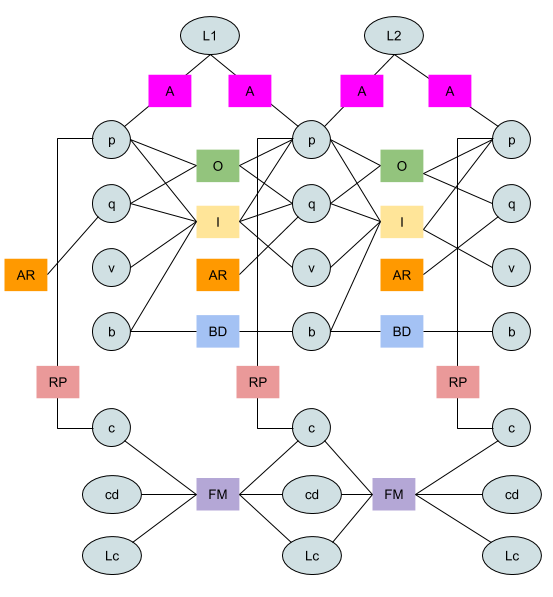
\includegraphics[width=0.7\linewidth]{img/IMU-Apriltag-Kinematics-Com.png}
    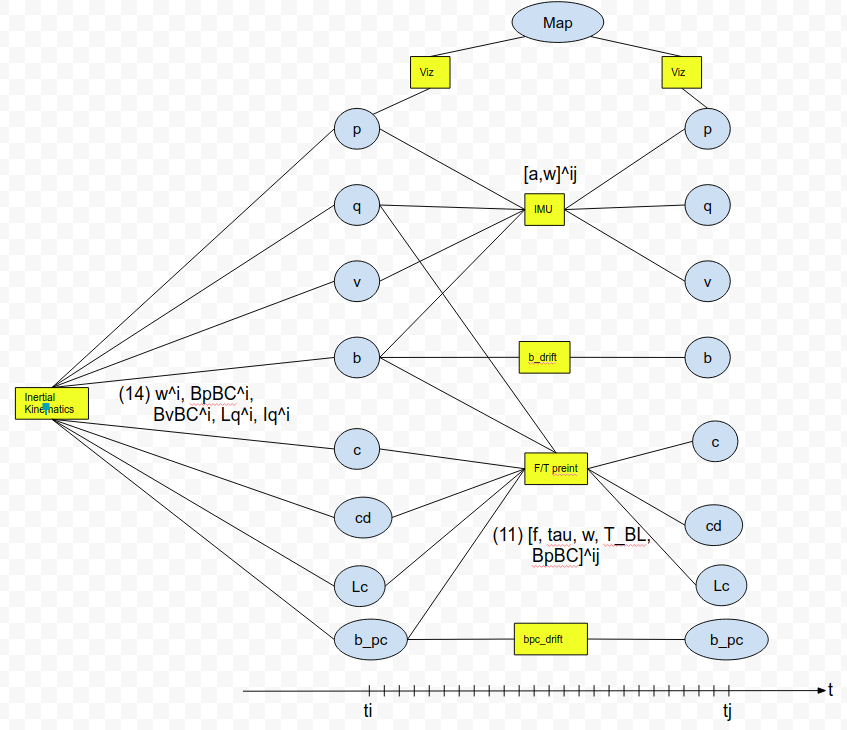
\includegraphics[width=1\linewidth]{img/HumanoidStateFactorGraph.png}
    % \caption{Factor graph representation of the simultaneous estimation of the robot state and COM state. Gray circles represent variables with from top to bottom Li: landmarks, p: robot position, q: robot orientation, v: robot velocity, b: IMU biases, c: COM position in foot frame, cd: COM velocity in foot frame, Lc: system angular momentum in foot frame. Constraints are represented as squares with A: Apriltag, O: odometry using forward kinematics, I: IMU, AR: absolute orientation, BD: bias drift, RP: relative position of the COM wrt. the robot reference frame, FM: force and moment measurements integration.}
    % \caption{Latest version at https://docs.google.com/drawings/d/1XQ80bcXe--4V49n_bDHHNxId_9YTiQ_YTVO0kwxaypA}
    \label{fig:my_label}
\end{figure}




















\section{Notations}
\begin{itemize}
    \item $\T{Y}{X}$: transformation SE(3) transformation so that $\prescript{Y}{}{v}=\T{Y}{X}\prescript{X}{}{v}$
    \item $\Tm{Y}{X}$: transformation measurement
    \item $C$: camera frame
    \item $K$: frame corresponding to the end of robot kinematic chain 
    \item $F$: one of the foot frame 
\end{itemize}

\begin{figure}[ht]
\begin{minipage}[c]{.46\linewidth}
    \centering
    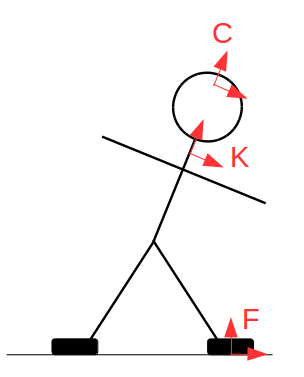
\includegraphics[width=0.6\linewidth]{img/robot_sketch.png}
    \label{fig:sketch}
    \caption{Frames diagram}
\end{minipage} \hfill
\begin{minipage}[c]{.46\linewidth}
    \centering
    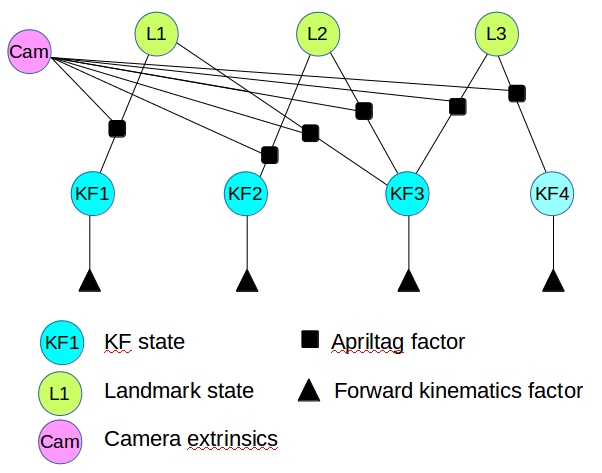
\includegraphics[width=\linewidth]{img/cam_extrinsics_factor_graph.png}
    \label{fig:factorgraph}
    \caption{Extrinsics calibration factor graph}
\end{minipage}
\end{figure}

























\section{Annexes}
\subsection{IMU pre-integration Delta derivation (Forster's)}
\subsubsection{Integration of pqv between distant timestamps}
State to estimate:

\begin{equation*}
\bfx = [\posi{W}{WB}, \vel{W}{WB}, \Rot{W}{B}, \bias_{\angvel{}{}}, \bias_{\bfa}]
\triangleq 
[\bfp, \bfv, \Rot{}{}, \bias_{\angvel{}{}}, \bias_{\bfa}] 
\end{equation*}

Continuous state space equations:

\begin{equation*}
\frac{d\posi{}{}}{dt} = \vel{}{}  ~~~~ \frac{d\vel{}{}}{dt} = \acc{W}{WB} ~~~~ \frac{d\Rot{}{}}{dt} = \Rot{}{} \angvel{B}{WB} 
\end{equation*}

Measurement model:

\begin{equation*}
\begin{split}
\angvelm{}{} &= \angvel{B}{WB} + \bias_{\angvel{}{}} + \noise_{\angvel{}{}} 
\\
\accm{}{}    &= \acc{B}{WB} + \bias_{\acc{}{}} + \noise_{\acc{}{}} 
\end{split}
\end{equation*}


Taylor type, zero hold on measurement integration during $dt = t_k - t_{k-1}$:

\begin{equation*}
\begin{split}
\Rot{}{}^{k+1}  &= \Rot{}{}^{k}Exp((\angvelm{}{}^k - \bias_{\angvel{}{}^k} - \noise_{\angvel{}{}^k})dt)
\\
\vel{}{}^{k+1}  &= \vel{}{}^{k} + \grav dt + \Rot{}{}^{k}(\accm{}{}^k - \bias_{\acc{}{}^k} - \noise_{\acc{}{}^k})dt
\\
\posi{}{}^{k+1} &= \posi{}{}^{k} + \vel{}{}^{k}dt + \frac{1}{2}\grav dt^2 
+ \frac{1}{2}\Rot{}{}^{k}(\accm{}{}^k - \bias_{\acc{}{}^k} - \noise_{\acc{}{}^k})dt^2
\end{split}
\end{equation*}


Summing from $k=i$ to $k=j-1$:

\begin{equation}
\begin{split}
\Rot{}{}^{j}  &= \Rot{}{}^{i} \prod_{k=i}^{j-1} Exp((\angvelm{}{}^k - \bias_{\angvel{}{}^k} - \noise_{\angvel{}{}^k})dt)
\\
\vel{}{}^{j}  &= \vel{}{}^{i} + \sum_{k=i}^{j-1} \Big[\grav dt + \Rot{}{}^{k}(\accm{}{}^k - \bias_{\acc{}{}^k} - \noise_{\acc{}{}^k})dt \Big]
\\
\posi{}{}^{j} &= \posi{}{}^{i} + \sum_{k=i}^{j-1} \Big[\vel{}{}^{k}dt + \frac{1}{2}\grav dt^2 
+ \frac{1}{2}\Rot{}{}^{k}(\accm{}{}^k - \bias_{\acc{}{}^k} - \noise_{\acc{}{}^k})dt^2 \Big]
\end{split}
\label{eq:IMUIntij}
\end{equation}

\subsubsection{Pre-interation formulas}
\textit{Quick def:} The goal is to define quantities that represent the movement of B relative to the time i so that those can be computed once and for all (except for bias adjustment, see later) by integrating measurements between i and j. We will proceed by rearranging the terms of \ref{eq:IMUIntij} to define these so called "delta quantities".

The rotation one is easy to get, multiplying by $\Rot{}{}^{i,T}$:
\begin{equation}
    \Delta R_{ij} \triangleq \Rot{}{}^{i,T} \Rot{}{}^{j} = \prod_{k=i}^{j-1} Exp((\angvelm{}{}^k - \bias_{\angvel{}{}^k} - \noise_{\angvel{}{}^k})dt)
    \label{eq:IMUDeltaR}
\end{equation}

The velocity is as well quite easy, by defining $\Delta t_{ij} \triangleq \sum_{k=i}^{j-1} dt = (j-i)dt$:
\begin{equation}
    \Delta v_{ij} \triangleq \Rot{}{}^{i,T} (\vel{}{j} - \vel{}{i} - g \Delta t_{ij}) 
    = \prod_{k=i}^{j-1} \Delta R_{ik} Exp((\accm{}{}^k - \bias_{\acc{}{}^k} - \noise_{\acc{}{}^k})dt)
    \label{eq:IMUDeltav}
\end{equation}

The position delta requires more calculations. First, inject equation \ref{eq:IMUDeltav} in the position equation of \ref{eq:IMUIntij} then rearrange and reorder the terms.

\begin{equation}
\begin{split}
\posi{}{}^{j} - \posi{}{}^{i} &= \sum_{k=i}^{j-1} \Big[
(\vel{}{}^i + \grav \Delta t_{ik} + \Rot{}{}^i \Delta v_{ik})dt 
+ \frac{1}{2}\grav dt^2 + \frac{1}{2}\Rot{}{}^{k}(\accm{}{}^k - \bias_{\acc{}{}^k} - \noise_{\acc{}{}^k})dt^2 \Big]
\\
&= \vel{}{}^i \Delta t_{ij} + 
\grav\sum_{k=i}^{j-1} \Delta t_{ik} dt + \frac{1}{2}\grav \sum_{k=i}^{j-1} dt^2 +
\Rot{}{}^i\sum_{k=i}^{j-1} \Big[\Delta v_{ik}dt +  \frac{1}{2} \Delta R_{ik} (\accm{}{}^k - \bias_{\acc{}{}^k} - \noise_{\acc{}{}^k})dt^2 \Big]
\\
&= \vel{}{}^i \Delta t_{ij} + 
\grav \sum_{k=i}^{j-1} (\Delta t_{ik} dt + \frac{1}{2}dt^2) +
\Rot{}{}^i\sum_{k=i}^{j-1} \Big[\Delta v_{ik}dt +  \frac{1}{2} \Delta R_{ik} (\accm{}{}^k - \bias_{\acc{}{}^k} - \noise_{\acc{}{}^k})dt^2 \Big]
\end{split}
\end{equation}

We will simplify the gravity term that we will call $\mathcal{G}t_{ij}$. Noting that:

\begin{equation*}
    \sum_{k=i}^{j-1}k = \sum_{k=1}^{j-1}k - \sum_{k=1}^{i-1}k = \frac{j(j-1)}{2} - \frac{i(i-1)}{2} 
\end{equation*}

we can deduce that:

\begin{equation*}
\begin{split}
\mathcal{G}t_{ij} 
&= dt \sum_{k=i}^{j-1}(\Delta t_{ik} + \frac{1}{2}dt) = dt \sum_{k=i}^{j-1}((k -i)dt + \frac{1}{2}dt)
\\
&= dt \Big[ \sum_{k=i}^{j-1} [ k dt - i(j-i)dt ] + \frac{1}{2}\Delta t_{ij}  \Big] 
\\
&= dt \Big[ \frac{dt}{2} (j(j-1) - i(i-1) - 2i(j-1)) + \frac{1}{2}\Delta t_{ij} \Big] 
\\
&= dt \Big[ \frac{dt}{2} (i^2 - 2ij + j^2 + i - j) + \frac{1}{2}\Delta t_{ij} \Big] 
\\
&= dt \Big[ \frac{1}{2} (j-i)^2dt - \frac{1}{2}(j - i)dt + \frac{1}{2}\Delta t_{ij} \Big]
\\
&= \frac{1}{2} (j-i)^2dt^2 = \frac{1}{2} \Delta t_{ij}^2
\end{split}
\end{equation*}
Multiplying by $\Rot{}{}^{i,T}$ and reordering the terms, we can finally define a position delta quantity:

\begin{equation}
    \Delta p_{ij} \triangleq \Rot{}{}^{i,T}(\posi{}{}^j - \posi{}{}^i - \vel{}{}^i \Delta t_{ij} - \frac{1}{2} \grav \Delta t_{ij}^2) = \sum_{k=i}^{j-1} \Big[\Delta v_{ik}dt +  \frac{1}{2} \Delta R_{ik} (\accm{}{}^k - \bias_{\acc{}{}^k} - \noise_{\acc{}{}^k})dt^2 \Big]
\end{equation}


\subsection{COM estimation misc notes}

Instead of using the biased kinematic measurement $\posim{B}{BC}$, we can 

\begin{equation}
\begin{split}
\frac{d\AM_c}{dt}&= \sum_l \Rot{}{}\Rot{B}{L}(q_A)(\torquem{}{l} - \noise_{\tau}) + (\bfp +
\Rot{}{}\posi{B}{BL}(q_A) - \COM)) \times \Rot{}{}\Rot{B}{L}(q_A)(\forcem{}{l} - \noise_f)
\end{split}
\label{eq:AMContinuousRandomNotes}
\end{equation}

First order discretization of \ref{eq:AMContinuousRandomNotes} gives:

\begin{equation}
\begin{split}
\AM_c^{k+1} &= \AM_c^{k} +  ( 
\sum_l \Rot{}{}^{k}\Rot{B}{L}^{k}(\torquem{}{l}^{k} - \noise_{\tau}^{k}) + (\bfp^{k-1} +
\Rot{}{}^{k}\posi{B}{BL}^{k} - \COM^{k})) \times \Rot{}{}^{k}\Rot{B}{L}^{k}(\forcem{}{l}^{k} - \noise_f^{k}) 
) \Delta t
\end{split}
\end{equation}



Adding measurements between 2 arbitrary timestamps \(t_i\) and \(t_j\) with \(\Delta t_{ij} \triangleq t_j - t_i\), we get the equations:

\begin{equation}
\begin{split}
\AM_c^{j} - \AM_c^{i} &=  \sum_{k=i}^{j-1} \Big[ 
\sum_l \Rot{B}{L}^{k-1} (\torquem{}{l}^{k} - \noise_{\tau}^{k} - (\forcem{}{l}^{k} - \noise_f^{k}) \times (\bfp^{k} + \Rot{}{}^{k}\posi{B}{BL}^{k} - \COM^{k})) \Big]  \Delta t
\end{split}
\end{equation}


for which preintegration equations are not obvious (in fact, they likely do not exist).



We can also derive the angular momentum equations in the inertial frame attached to one of the extremities in contact (the one that we trust the most maybe). We will only write the case where only one of the extremities is in contact: \(l*\).

\begin{equation}
\begin{split}
    \frac{d \prescript{L*}{}{\AM}_c}{dt} &=
    (\torquem{}{l} - \noise_{\tau}) + \posi{L*}{CL*}(q_A) \times (\forcem{}{l*} - \noise_f)
    \\
    &= (\torquem{}{l} - \noise_{\tau}) + (\Rot{L*}{B}(q_A)\Rot{}{}^T(\bfp - \COM) + \posi{L*}{BL*}(q_A)) \times (\forcem{}{l*} - \noise_f)
\end{split}
\end{equation}
 
but again this leads to untangled equations that cannot be pre-integrated.



\printbibliography



\end{document}






